\newpage
\section{Auswertung}
\label{sec:Auswertung}

\subsection{Temperaturverläufe}
    Die Temperaturverläufe in Abbildung \ref{fig:plot_temp}, Werte angehängt (siehe {\ref{messwerte}).
    \begin{figure}
        \centering
        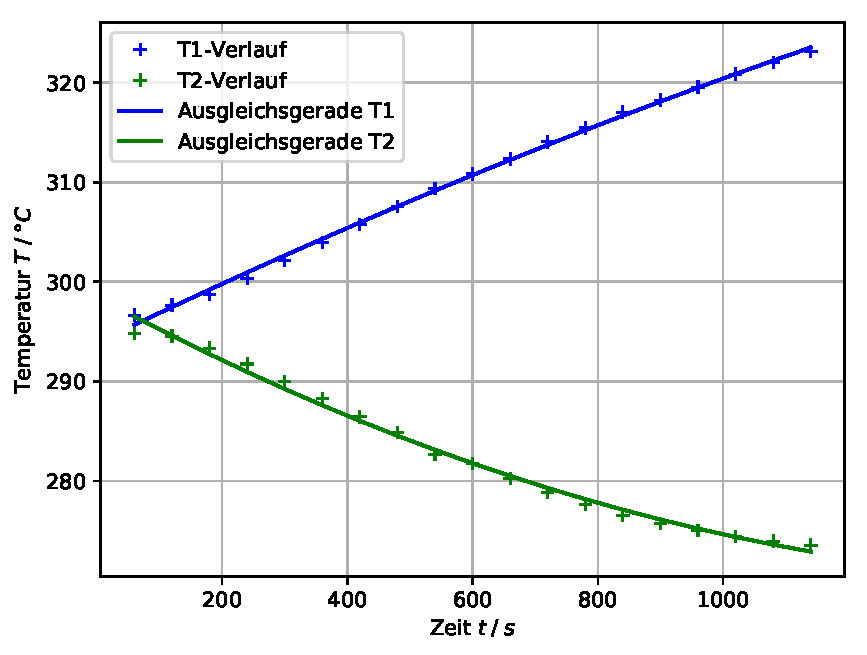
\includegraphics[width=\textwidth]{build/plot_temp.pdf}
        \caption{Temperaturverläufe}
        \label{fig:plot_temp}
    \end{figure}

\subsection{Nicht-lineare Ausgleichsrechnung}
    Mit der folgenden Näherung, werden nun die in \ref{fig:plot_temp}
    dargestellten Ausgleichsgeraden bestimmt\cite{curvefit}:
    \begin{equation}
        T(t)=At^2+Bt+C
        \label{eqn:ausgleichsgerade}
    \end{equation}
    \begin{table}
        \centering
        \begin{tabular}{c || c | c}
            \toprule
            & $T_1\;/\;K$ & $T_2\;/\;K$ \\
            \midrule
            A\;/\;$K/s^2$& $(-3,8\pm0,9)\;10^{-6}$ & $(1,01\pm0,16)\;10^{-5}$ \\
            B\;/\;$K/s$& 0,0304\pm0,0012 & -0,0339\pm0,0019 \\
            C\;/\;$K$& 293,88\pm0,30 & 298,5\pm0,5 \\
            \bottomrule
        \end{tabular}
    \end{table}
\subsection{Differentialquotienten}
    Exemplarisch werden für vier Messwerte der Differentialquotienten $dT1/dt$ und
    $dT2/dt$ berechnet.
    Für die Näherung von \eqref{eqn:ausgleichsgerade} folgt somit:
    \begin{equation}
        \frac{dT}{dt}=2At+Bt
    \end{equation}
    mit einem Fehler nach Gaußscher Fehlerfortpflanzung.\\
    Es ergeben sich die vier verschieden Differenialquotienten
    \begin{table}
        \centering
        \begin{tabular}{c c c}
            \toprule
            Zeit $T\;/\;s$ & $T_1$ & d$T_1$/d$t$ \\
            \midrule
            240,0 & 300,35 & 0,0285\pm0,0012\\
            480,0 & 307,55 & 0,0267\pm0,0015 \\
            840,0 & 317,045 & 0,0239\pm0,0020  \\
            1080,0 & 322,045 & 0,0221\pm0,0023\\
            \midrule
            Mittelwert &&  0.0253\pm0.0017  \\
            \bottomrule
        \end{tabular}
        \caption{Differentialquotienten für $T_1$}
        \label{fig:tab_T1t}
    \end{table}

    \begin{table}
        \centering
        \begin{tabular}{c c c c}
            \toprule
            Zeit $T\;/\;s$ & $T_2$ & d$T_2$/d$t$ \\
            \midrule
            240,0 & 291,75 & -0,029 \\
            480,0 & 284,85 & -0,024 \\
            840,0 & 276,55 & -0,017 \\
            1080,0 & 273,95 & -0,012 \\
            \midrule
            Mittelwert &&  -0,021 \\
            \bottomrule
        \end{tabular}
        \caption{Differentialquotienten für $T_2$}
        \label{fig:tab_T2t}
    \end{table}
    \newpage
    \subsection{Bestimmung der Güteziffer}
    Wie in Gleichung (\ref{eqn:nu_ideal}) dargestellt, lässt sich aus dem zuvor berechneten
    Differentialquotienten die Güteziffer $\nu$ bestimmen.\\
    Für die Wärmekapazität von Wasser $m_1\;c_w$ und von Kupfer $m_k\;c_k$ gilt gilt \cite{wasser}:
    \begin{align*}
        m_1\;c_w &= 4190\frac{J}{kg\;K} 	\Rightarrow 12570\frac{J}{K}\\
        m_k\;c_k &= 750\frac{J}{K}
    \end{align*}

    \begin{table}
        \centering
        \begin{tabular}{c c c c}
        \toprule
        Zeit $t\;/\;s$ & Güteziffer $v_{ideal}$ & Güteziffer $v_{real}$&Abweichung / \%\\
        \midrule
        120,0 & 96,02 & 1,97\pm0,08   &97,9  \\
        480,0 & 24,77 & 1,87\pm0,09   &92,43 \\
        840,0 & 7,83 & 1,60\pm0,13    &79,6  \\
        1140,0 & 6,56 & 1,45\pm0,16   &77,8   \\
        \end{tabular}
    \end{table}
    
%%%%%%%%%%%%%%%%%%%%%%%%%%%%%%%%%%%%%%%%%%%%%%%%%%%%%%%%%

\subsection{Massendurchsatz}
Zuerst wird die Verdampfungswärme mithilfe einer linearen Regression wie in Versuch 203 bestimmt.
Die Ausgleichskurve wird über den folgenden Zusammenhang gebildet.
\begin{align*}
    \ln(\frac{p}{p_0})&= -\frac{L}{R}\cdot\frac{1}{T}\\
    \ln(p)&=-\frac{L}{R}\frac{1}{T}+b \\
    \Rightarrow ln(p)&=-a\frac{1}{T}+b    
\end{align*}
Über die Parameter
\begin{align*}
  \symup{m} &= 2237\pm76K \\
  \symup{b} &= 8,06\pm0,25 \:
\end{align*}
lässt sich dann L bestimmen.
\begin{align*}
    L &= m\cdot R\\
    %L &= 18604,98 \pm 0,25
\end{align*}
Dividiere dies durch die molare Masse von $Cl_2F_2C=120\frac{g}{mol}$ 
so ergibt sich die Einheit $\frac{J}{g}$.
\begin{equation*}
    L=(154\pm5) \;\frac{J}{g}
\end{equation*}
\begin{figure}[H]
  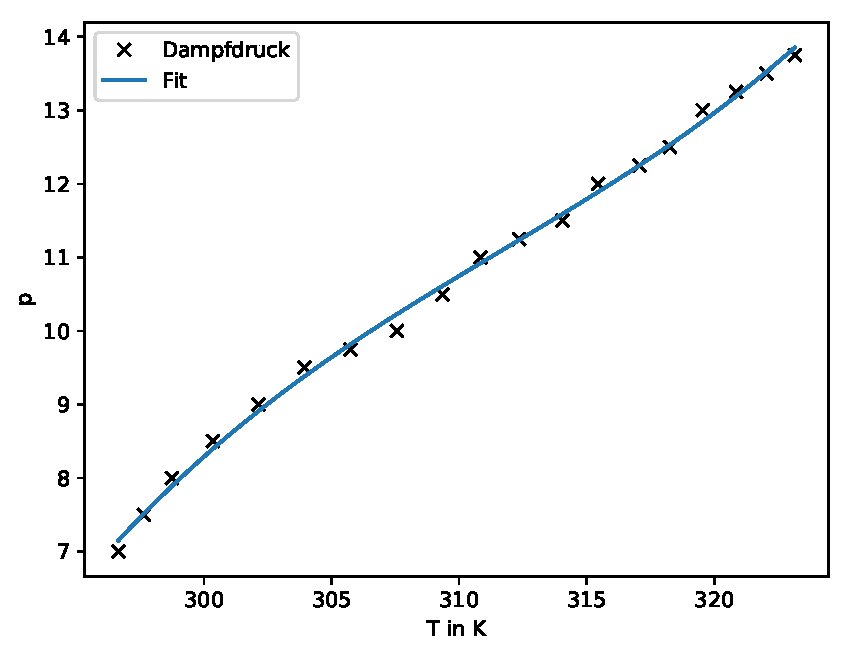
\includegraphics{build/plot_L.pdf}
  \caption{Dampfdruckkurve für $\symup{P}$ und $\symup{T}$ im warmen Reservoir.}
  \label{fig:Dampfp}
\end{figure}
Die Unsicherheit ergibt sich mit der Gauß'schen Fehlerfortpflanzung.
Mit dem so erhaltenen Wert für $L$ wird nun der Massendurchsatz bestimmt.
\begin{equation*}
    \frac{\symup{d}m}{\symup{d}t} = \frac{\nu_{real}\cdot N}{L}
\end{equation*}
Der Massendurchsatz $\symup{d}m / \symup{d}t$ an der jeweiligen Messstelle ist
in Tabelle \ref{tab:massendurch} aufgeführt.
\begin{table}[H]
        \centering
        \begin{tabular}{c c}
        \toprule
        Zeit $t\;/\;s$ & Massendurchsatz in $\frac{dm}{dt}\;/\; g/s$ \\
        \midrule
        120.0 & 2.55\pm0.13\\
        480.0 & 2.43\pm0.14\\
        840.0 & 2.07\pm0.18 \\
        1140.0 & 1.87\pm0.22 \\
        \end{tabular}
        \caption{Massendurchsatz}
        \label{tab:massendurch}
    \end{table}
\newpage
\subsection{Mechanische Kompressionsleistung}
Die mechanische Kompressionsleistung bestimmt sich über \ref{eqn:kompress2}
Die Dichte des Mediums bei der vorligenden Temperatur lässt
sich aus der idealen Gasgleichung bestimmen.
\begin{equation*}
    \frac{p_0V_0}{T_0}=\frac{pV}{T}
\end{equation*}
Es folgt:
\begin{equation}
    \rho=\frac{p \rho_0 T_0}{p_0 T}
\end{equation}
mit $\rho_0(Cl_2F_2C)=5,51g/l$ und $\kappa=1,14$ folgt:
\begin{table}[H]
        \centering
        \begin{tabular}{c c c}
        \toprule
        Zeit $t\;/\;$s & $\rho\;/\; kg/m^3$ & Kompressorleistung $N_{mech}\;/\;$ W \\
        \midrule
        120.0 & 3.01 &2.18\pm0.11\\
        480.0 & 3.56 &2.11\pm0.12\\
        840.0 & 4.62  &1.84\pm0.16 \\
        1140.0 & 5.09 &1.65\pm0.19 \\

        \end{tabular}
        \caption{Kompressorleistung}
        \label{tab:kompress}
    \end{table}